\begin{flushright} {\tiny {\color{gray} \tt elements3D.tex}} \end{flushright}
%~~~~~~~~~~~~~~~~~~~~~~~~~~~~~~~~~~~~~~~~~~~~~~~~~~~~~~~~~~~~~~~~~~~~~~~~~~~~~~~~~~~~~~~~~~~~~~~~~~

%%%%%%%%%%%%%%%%%%%%%%%%%%%%%%%%%%%%%%%%%%%%%%%%%%%%%%%%%%%%%%%%%%%%%%%%%%%%%%%
\subsection{Trilinear basis functions ($Q_1$)}
\index{general}{$Q_1$}
Following Section~\ref{ss:q12d}, we can simply write:

\begin{mdframed}[backgroundcolor=blue!5]
\begin{eqnarray}
\bN_1(r,s,t)&=&0.125(1-r)(1-s)(1-t) \nn\\ 
\bN_2(r,s,t)&=&0.125(1+r)(1-s)(1-t) \nn\\ 
\bN_3(r,s,t)&=&0.125(1+r)(1+s)(1-t) \nn\\ 
\bN_4(r,s,t)&=&0.125(1-r)(1+s)(1-t) \nn\\ 
\bN_5(r,s,t)&=&0.125(1-r)(1-s)(1+t) \nn\\ 
\bN_6(r,s,t)&=&0.125(1+r)(1-s)(1+t) \nn\\ 
\bN_7(r,s,t)&=&0.125(1+r)(1+s)(1+t) \nn\\ 
\bN_8(r,s,t)&=&0.125(1-r)(1+s)(1+t) \nn
\end{eqnarray}
\end{mdframed}
These basis functions are the product of the linear basis functions of Section~\ref{sec:bf1}.

\begin{center}
\begin{flushright} {\tiny {\color{gray} \tt (tikz\_q1.tex)}} \end{flushright}
%~~~~~~~~~~~~~~~~~~~~~~~~~~~~~~~~~~~~~~~~~~~~~~~~~~~~~~~~~~~~~~~~~~~~~~~~~~~~~~~~~~~~~~~~~~~~~~~~~~

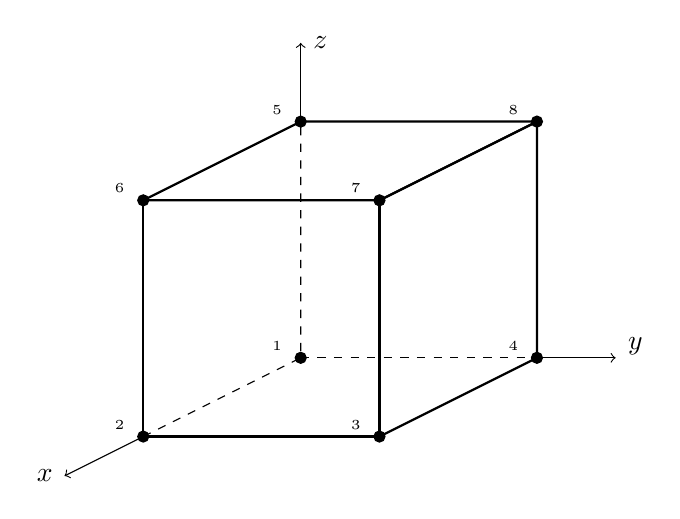
\begin{tikzpicture}
%\draw[fill=gray!23,gray!23](0,0) rectangle (9,7);
%\draw[step=0.5cm,gray,very thin] (0,0) grid (9,7); %background grid

\draw[thick] (2,4.5) -- (5,4.5) -- (7,5.5) -- (4,5.5) -- cycle; %top
\draw[thick] (2,1.5) -- (5,1.5) -- (5,4.5) -- (2,4.5) -- cycle; %front
\draw[thick] (5,1.5) -- (7,2.5) -- (7,5.5) -- (5,4.5) -- cycle; %right

\draw[dashed]   (2,1.5) -- (4,2.5) -- (4,5.5) ; % 
\draw[dashed]   (4,2.5) -- (7,2.5)  ; % 

\draw[thin,->] (2,1.5) -- (1,1); %x
\draw[thin,->] (7,2.5) -- (8,2.5); %y
\draw[thin,->] (4,5.5) -- (4,6.5); %z
\node[] at (0.75,1) {$x$};
\node[] at (8.25,2.65) {$y$};
\node[] at (4.25,6.5) {$z$};

\draw[black,fill=black] (4,2.5)   circle (2pt);
\draw[black,fill=black] (2,1.5)   circle (2pt);
\draw[black,fill=black] (7,2.5)   circle (2pt);
\draw[black,fill=black] (5,1.5)   circle (2pt);
\draw[black,fill=black] (4,5.5)   circle (2pt);
\draw[black,fill=black] (2,4.5)   circle (2pt);
\draw[black,fill=black] (7,5.5)   circle (2pt);
\draw[black,fill=black] (5,4.5)   circle (2pt);

\node[] at (3.7,2.65) {\tiny 1};
\node[] at (1.7,1.65) {\tiny 2};
\node[] at (6.7,2.65) {\tiny 4};
\node[] at (4.7,1.65) {\tiny 3};

\node[] at (3.7,5.65) {\tiny 5};
\node[] at (1.7,4.65) {\tiny 6};
\node[] at (6.7,5.65) {\tiny 8};
\node[] at (4.7,4.65) {\tiny 7};
\end{tikzpicture}


\end{center}
Note that the figure above depicts an element in $x,y,z$ space, not the reference
element in $r,s,t$ space which is centered around the origin.


%%%%%%%%%%%%%%%%%%%%%%%%%%%%%%%%%%%%%%%%%%%%%%%%%%%%%%%%%%%%%%%%%%%%%%%%%%%%%%%
\subsection{Triquadratic basis functions ($Q_2$)}
\index{general}{$Q_2$}
\begin{flushright} {\tiny {\color{gray} basis\_q2\_3D.tex}} \end{flushright}
%~~~~~~~~~~~~~~~~~~~~~~~~~~~~~~~~~~~~~~~~~~~~~~~~~~~~~~~~~~~~~~~~~~~~~~~~~~~~~~~~~~~~~~~~~~~~~~~~~~

\begin{center}
\input{tikz/tikz_q2}
\end{center}
Note that the figure above depicts an element in $x,y,z$ space, not the reference
element in $r,s,t$ space which is centered around the origin.

\begin{eqnarray}
\bN_{1} &=& 0.5r(r-1)  \cdot 0.5s(s-1) \cdot 0.5t(t-1) \nn\\
\bN_{2} &=& (1-r^2)    \cdot 0.5s(s-1) \cdot 0.5t(t-1) \nn\\
\bN_{3} &=& 0.5r(r+1)  \cdot 0.5s(s-1) \cdot 0.5t(t-1) \nn\\
\bN_{4} &=&  0.5r(r-1) \cdot (1-s^2)   \cdot 0.5t(t-1) \nn\\
\bN_{5} &=&  (1-r^2)   \cdot (1-s^2)   \cdot 0.5t(t-1) \nn\\
\bN_{6} &=& 0.5r(r+1)  \cdot (1-s^2)   \cdot 0.5t(t-1) \nn\\
\bN_{7} &=&  0.5r(r-1) \cdot 0.5s(s+1) \cdot 0.5t(t-1) \nn\\
\bN_{8} &=&  (1-r^2)   \cdot 0.5s(s+1) \cdot 0.5t(t-1) \nn\\
\bN_{9} &=& 0.5r(r+1)  \cdot 0.5s(s+1) \cdot 0.5t(t-1) \nn\\
\bN_{10}&=&  0.5r(r-1) \cdot 0.5s(s-1) \cdot (1-t^2) \nn\\
\bN_{11}&=&  (1-r^2)   \cdot 0.5s(s-1) \cdot (1-t^2) \nn\\
\bN_{12}&=& 0.5r(r+1)  \cdot 0.5s(s-1) \cdot (1-t^2) \nn\\
\bN_{13}&=&  0.5r(r-1) \cdot (1-s^2)   \cdot (1-t^2) \nn\\
\bN_{14}&=&  (1-r^2)   \cdot (1-s^2)   \cdot (1-t^2) \nn\\
\bN_{15}&=& 0.5r(r+1)  \cdot (1-s^2)   \cdot (1-t^2) \nn\\
\bN_{16}&=&  0.5r(r-1) \cdot 0.5s(s+1) \cdot (1-t^2) \nn\\
\bN_{17}&=&  (1-r^2)   \cdot 0.5s(s+1) \cdot (1-t^2) \nn\\
\bN_{18}&=& 0.5r(r+1)  \cdot 0.5s(s+1) \cdot (1-t^2) \nn\\
\bN_{19}&=&  0.5r(r-1) \cdot 0.5s(s-1) \cdot 0.5t(t+1) \nn\\
\bN_{20}&=&  (1-r^2)   \cdot 0.5s(s-1) \cdot 0.5t(t+1) \nn\\
\bN_{21}&=& 0.5r(r+1)  \cdot 0.5s(s-1) \cdot 0.5t(t+1) \nn\\
\bN_{22}&=&  0.5r(r-1) \cdot (1-s^2)   \cdot 0.5t(t+1) \nn\\
\bN_{23}&=&  (1-r^2)   \cdot (1-s^2)   \cdot 0.5t(t+1) \nn\\
\bN_{24}&=& 0.5r(r+1)  \cdot (1-s^2)   \cdot 0.5t(t+1) \nn\\
\bN_{25}&=&  0.5r(r-1) \cdot 0.5s(s+1) \cdot 0.5t(t+1) \nn\\
\bN_{26}&=&  (1-r^2)   \cdot 0.5s(s+1) \cdot 0.5t(t+1) \nn\\
\bN_{27}&=& 0.5r(r+1)  \cdot 0.5s(s+1) \cdot 0.5t(t+1) \nn
\end{eqnarray}








%%%%%%%%%%%%%%%%%%%%%%%%%%%%%%%%%%%%%%%%%%%%%%%%%%%%%%%%%%%%%%%%%%%%%%%%%%%%%%%
\subsection{Linear basis functions in tetrahedra ($P_1$)}
\index{general}{$P_1$}
\input{basis_p1_3D}

%%%%%%%%%%%%%%%%%%%%%%%%%%%%%%%%%%%%%%%%%%%%%%%%%%%%%%%%%%%%%%%%%%%%%%%%%%%%%%%
\subsection{Enriched linear in tetrahedra($P_1^+$)}
\index{general}{$P_1^+$}
\input{basis_p1p_3D}

%%%%%%%%%%%%%%%%%%%%%%%%%%%%%%%%%%%%%%%%%%%%%%%%%%%%%%%%%%%%%%%%%%%%%%%%%%%%%%%
\subsection{Enriched quadratic basis functions in tetrahedra ($P_2^+$)}
\index{general}{$P_2^+$}
\input{basis_p2p_3D}

%%%%%%%%%%%%%%%%%%%%%%%%%%%%%%%%%%%%%%%%%%%%%%%%%%%%%%%%%%%%%%%%%%%%%%%%%%%%%%%
%.....................................................................
\subsection{Linear basis functions for hexahedra ($P_{-1}$)} \label{ss:lbfh3D}
\index{general}{$P_1$}

This is the ${\bm Q}_2\times P_{-1}$ element. 
I choose the reduced coordinates of the pressure nodes to be :

\begin{tabular}{cccc}
\hline
point & r & s & t \\
\hline
1& 1/2 &-1/2 &-1/2\\
2& -1/2 &1/2 &-1/2\\
3& -1/2 &-1/2& 1/2\\
4& 1/2 &1/2& 1/2 \\
\hline
\end{tabular}

Inside the element the pressure is given as a linear function of the reduced coordinates $r,s,t$:
\[
p(r,s,t)=a+br+cs+dt
\]
This expression must exactly interpolate the pressure at all four pressure nodes:
\begin{eqnarray}
p_1 
&=& p(r_1,s_1,t_1) 
= a+br_1+cs_1+dt_1 
= a+b/2-c/2-d/2\nonumber\\
p_2
&=& p(r_2,s_2,t_2)
= a+br_2+cs_2+dt_2
= a-b/2+c/2-d/2\nonumber\\
p_3
&=& p(r_3,s_3,t_3) 
= a+br_3+cs_3+dt_3 
= a-b/2-c/2+d/2\nonumber\\
p_4
&=& p(r_4,s_4,t_4) 
= a+br_4+cs_4+dt_4
= a+b/2+c/2+d/2\nonumber
\end{eqnarray}
or,
\begin{equation}
\left(
\begin{array}{cccc}
1 & 1/2 & -1/2 & -1/2 \\
1 & -1/2 & +1/2 & -1/2 \\
1 & -1/2 & -1/2 & +1/2 \\
1 & 1/2 & +1/2 & +1/2 
\end{array}
\right)
\left(
\begin{array}{c}
a\\b\\c\\d
\end{array}
\right)=
\left(
\begin{array}{c}
p_1\\p_2\\p_3\\p_4
\end{array}
\right)
\nonumber
\end{equation}

The matrix is invertible and we get:
\[
\left(
\begin{array}{c}
a\\b\\c\\d
\end{array}
\right)=
\left(
\begin{array}{cccc}
1/4 & 1/4 & 1/4 & 1/4 \\
1/2 & -1/2 & -1/2 & 1/2 \\
-1/2 & 1/2 & -1/2 & 1/2 \\
-1/2 & -1/2 & 1/2 & 1/2
\end{array}
\right)
\left(
\begin{array}{c}
p_1\\p_2\\p_3\\p_4
\end{array}
\right)
\]

so 
\begin{eqnarray}
p(r,s,t)
&=& a+br+cs+dt \nonumber\\
&=& \frac{1}{4}(p_1+p_2+p_3+p_4)
+\frac{1}{2}(p_1-p_2-p_3+p_4)r
+\frac{1}{2}(-p_1+p_2-p_3+p_4)s
+\frac{1}{2}(-p_1-p_2+p_3+p_4)t\nonumber\\
&=&
\frac{1}{4}(1+2r-2s-2t)p_1+
\frac{1}{4}(1-2r+2s-2t)p_2+
\frac{1}{4}(1-2r-2s+2t)p_3+
\frac{1}{4}(1+2r+2s+2t)p_4 \nonumber\\
&=& \sum_{i=1}^4 N_i(r,s,t) p_i
\end{eqnarray}
with
\begin{eqnarray}
N_1(r,s,t) &=& \frac{1}{4}(1+2r-2s-2t)\nonumber\\
N_2(r,s,t) &=& \frac{1}{4}(1-2r+2s-2t)\nonumber\\
N_3(r,s,t) &=& \frac{1}{4}(1-2r-2s+2t)\nonumber\\
N_4(r,s,t) &=& \frac{1}{4}(1+2r+2s+2t)\nonumber
\end{eqnarray}

\vspace{.6cm}

I could also have chosen 

\begin{tabular}{cccc}
\hline
point & r & s & t \\
\hline
1& 0 & 0 &0 \\
2& 1 & 0 &0 \\
3& 0 & 1 &0 \\
4& 0 & 0 &1 \\
\hline
\end{tabular}

This expression must exactly interpolate the pressure at all four pressure nodes:
\begin{eqnarray}
p_1  &=& p(r_1,s_1,t_1) = a+br_1+cs_1+dt_1 = a\nonumber\\
p_2  &=& p(r_2,s_2,t_2) = a+br_2+cs_2+dt_2 = a+b\nonumber\\
p_3  &=& p(r_3,s_3,t_3) = a+br_3+cs_3+dt_3 = a+c\nonumber\\
p_4  &=& p(r_4,s_4,t_4) = a+br_4+cs_4+dt_4 = a+d\nonumber
\end{eqnarray}
i.e.
\[
a=p_1
\qquad
b=p_2-p1
\qquad
c=p_3-p1
\qquad
d=p_4-p1
\]
or, 
\[
p^h(r,s)=a+br+cs+dt=p_1 + (p_2-p_1)r + (p_3-p_1)r + (p_4-p_1)t  = p_1(1-r-s-t) + r p_2 + s p_3 + t p_4
\]
so 
\begin{mdframed}[backgroundcolor=blue!5]
\begin{eqnarray}
N_1(r,s,t) &=& 1-r-s-t \\ 
N_2(r,s,t) &=& r \\
N_3(r,s,t) &=& s \\
N_4(r,s,t) &=& t
\end{eqnarray}
\end{mdframed}






%%%%%%%%%%%%%%%%%%%%%%%%%%%%%%%%%%%%%%%%%%%%%%%%%%%%%%%%%%%%%%%%%%%%%
\subsection{20-node serendipity basis functions in 3D ($Q_2^{(20)}$)}
\index{general}{$Q_2^{(20)}$} \index{general}{Serendipity element}

The serendipity elements are those rectangular elements which have no
interior nodes \cite[p91]{reddybook2}.

\begin{verbatim}
   t
   |
   .--s
  /
 r
                                    05=====20=====08 
                                    |             |  
                                    |             |  
                  17 - - - - - -19  13            16
                  .              .  |             |  
                  .              .  |             |  
06=====18=====07  .              .  01=====12=====04 @ r=-1
|             |   .              . 
|             |   .              .  
14            15  09 - - - - - -11 @ r=0
|             |   
|             |  
02=====10=====03 @ r=+1
\end{verbatim}

\todo[inline]{find/build basis functions!}


%..........................................................................---------------------------
%\subsection{Enriched linear basis functions in quadrilaterals ($Q_1^+$) -WIP} \label{ss:quadmini3D}
%\index{general}{$Q_1^+$}

%\input{lamichhane3D}


%-----------------------------------------------------------------
\subsection{The rotated $Q_1$} \label{ss:rq1_3D}
\index{general}{$\tilde{Q}_1$}

The nodes are not on the corners of the element but in the middle of the
element faces:

\begin{center}
\includegraphics[width=4cm]{images/rannacherturek/elt3D}\\
{\captionfont Node numbering and connectivity pattern of the reference element. Taken from \cite{gekm08}}
\end{center}

We have $\tilde{Q}_1=span \{1,r,s,t,r^2-s^2,s^2-t^2\}$.

%.............................................
\paragraph{The Middle Point (MP) variant}. 

The basis functions are given by (see Georgiev \etal (2008) \cite{gekm08}):
\begin{eqnarray}
N_1(r,s,t) &=& \frac{1}{6}(1-3r+2r^2-s^2-t^2 ) \\
N_2(r,s,t) &=& \frac{1}{6}(1+3r+2r^2-s^2-t^2 ) \\
N_3(r,s,t) &=& \frac{1}{6}(1-r^2-3s+2s^2-t^2 ) \\
N_4(r,s,t) &=& \frac{1}{6}(1-r^2+3s+2s^2-t^2 ) \\
N_5(r,s,t) &=& \frac{1}{6}(1-r^2-s^2-3t+2t^2 ) \\
N_6(r,s,t) &=& \frac{1}{6}(1-r^2-s^2+3t+2t^2 ) 
\end{eqnarray}

\begin{eqnarray}
\frac{\partial N_1}{\partial r} &=& \frac{1}{6} (-3+4r )\\
\frac{\partial N_2}{\partial r} &=& \frac{1}{6} (3+4r )\\
\frac{\partial N_3}{\partial r} &=& \frac{1}{6} (-2r) \\
\frac{\partial N_4}{\partial r} &=& \frac{1}{6} (-2r) \\
\frac{\partial N_5}{\partial r} &=& \frac{1}{6} (-2r) \\
\frac{\partial N_6}{\partial r} &=& \frac{1}{6} (-2r) 
\end{eqnarray}

\begin{eqnarray}
\frac{\partial N_1}{\partial s} &=& \frac{1}{6} (-2s)\\ 
\frac{\partial N_2}{\partial s} &=& \frac{1}{6} (-2s) \\
\frac{\partial N_3}{\partial s} &=& \frac{1}{6} (-3+4s )\\
\frac{\partial N_4}{\partial s} &=& \frac{1}{6} (3+4s )\\
\frac{\partial N_5}{\partial s} &=& \frac{1}{6} (-2s) \\
\frac{\partial N_6}{\partial s} &=& \frac{1}{6} (-2s) 
\end{eqnarray}

\begin{eqnarray}
\frac{\partial N_1}{\partial t} &=& \frac{1}{6}(-2t) \\ 
\frac{\partial N_2}{\partial t} &=& \frac{1}{6}(-2t) \\ 
\frac{\partial N_3}{\partial t} &=& \frac{1}{6}(-2t) \\ 
\frac{\partial N_4}{\partial t} &=& \frac{1}{6}(-2t) \\ 
\frac{\partial N_5}{\partial t} &=& \frac{1}{6}(-3+4t) \\ 
\frac{\partial N_6}{\partial t} &=& \frac{1}{6}(3+4t)  
\end{eqnarray}


%......................................
\paragraph{The Mid Value (MV) variant}. 

\begin{eqnarray}
N_1(r,s,t) &=& \frac{1}{12}(2-6r+6r^2-3s^2-3t^2) \\
N_2(r,s,t) &=& \frac{1}{12}(2+6r+6r^2-3s^2-3t^2) \\
N_3(r,s,t) &=& \frac{1}{12}(2-3r^2-6s+6s^2-3t^2) \\
N_4(r,s,t) &=& \frac{1}{12}(2-3r^2+6s+6s^2-3t^2) \\
N_5(r,s,t) &=& \frac{1}{12}(2-3r^2-3s^2-6t+6t^2) \\
N_6(r,s,t) &=& \frac{1}{12}(2-3r^2-3s^2+6t+6t^2)
\end{eqnarray}

\begin{eqnarray}
\frac{\partial N_1}{\partial r} &=& \frac{1}{12}(-6+12r) = \frac{1}{2}(-1+2r)\\
\frac{\partial N_2}{\partial r} &=& \frac{1}{12}(6+12r) = \frac{1}{2}(1+2r)\\
\frac{\partial N_3}{\partial r} &=& \frac{1}{12}(-6r) = -\frac{1}{2}r \\
\frac{\partial N_4}{\partial r} &=& \frac{1}{12}(-6r) = -\frac{1}{2}r \\
\frac{\partial N_5}{\partial r} &=& \frac{1}{12}(-6r) = -\frac{1}{2}r \\
\frac{\partial N_6}{\partial r} &=& \frac{1}{12}(-6r) = -\frac{1}{2}r 
\end{eqnarray}

\begin{eqnarray}
\frac{\partial N_1}{\partial s} &=& \frac{1}{12} (-6s) = -\frac{1}{2}s \\
\frac{\partial N_2}{\partial s} &=& \frac{1}{12} (-6s) = -\frac{1}{2}s \\
\frac{\partial N_3}{\partial s} &=& \frac{1}{12} (-6+12s) = \frac{1}{2} (-1+2s) \\ 
\frac{\partial N_4}{\partial s} &=& \frac{1}{12} (6+12s) = \frac{1}{2} (1+2s) \\ 
\frac{\partial N_5}{\partial s} &=& \frac{1}{12} (-6s) = -\frac{1}{2}s \\
\frac{\partial N_6}{\partial s} &=& \frac{1}{12} (-6s) = -\frac{1}{2}s 
\end{eqnarray}

\begin{eqnarray}
\frac{\partial N_1}{\partial t} &=& \frac{1}{12} (-6t) = -\frac{1}{2}t \\
\frac{\partial N_2}{\partial t} &=& \frac{1}{12} (-6t) = -\frac{1}{2}t \\
\frac{\partial N_3}{\partial t} &=& \frac{1}{12} (-6t) = -\frac{1}{2}t \\
\frac{\partial N_4}{\partial t} &=& \frac{1}{12} (-6t) = -\frac{1}{2}t \\
\frac{\partial N_5}{\partial t} &=& \frac{1}{12} (-6+12t) = \frac{1}{2} (-1+2t) \\ 
\frac{\partial N_6}{\partial t} &=& \frac{1}{12} (6+12t) = \frac{1}{2} (1+2t) 
\end{eqnarray}



